\documentclass{article}
\usepackage{amsmath}
\usepackage{amssymb}
\usepackage{pgfplots}
\usepackage{graphicx}
\pgfplotsset{compat=1.16}

\title{\textbf{Assignment 5 Q53 (june 2018)}}
\author{Abhishek Ajit Sabnis}
\date{28 February 2022}

\begin{document}

\maketitle

\textbf{53) Suppose that the lifetime of an electric bulb follows an exponential distribution with mean $\theta$ hours. In order to estimate $\theta$, n bulbs are switched on at the same time. After t hours, n-m($>$0) bulbs are found in functioning state. If the lifetimes of other m($>$0) bulbs are noted as $x_1, x_2,....,x_m$ respectively, then the maximum likelihood estimate of $\theta$ is given by  }

\vspace{0.5cm}

\textbf{Ans} 

Probability distribution function of Exponential distribution is given by - 
\begin{equation}
    f_X(x) = \lambda e^{-\lambda x}
\end{equation}

Given mean is $\theta$. We know
\begin{equation}
    E(X) = \frac{1}{\lambda} = \theta
\end{equation}

Substitute in eq(1) we get,
\begin{equation}
    f_X(x) = \frac{1}{\theta} e^{-\frac{x}{\theta}}
\end{equation}

\textbf{Likelihood function -}

\begin{equation}
    L(x_1,....x_n) = \prod f_X(x_i) = (\frac{1}{\theta})^n exp(\frac{-1}{\theta} \sum_{i=1}^{n} x_i)
\end{equation}

Take logarithm of the likelihood function - 

\begin{equation}
    log(L) = l = n log(\frac{1}{\theta}) - \frac{1}{\theta} \sum_{i=1}^{n} x_i
\end{equation}

Maximizing the log likelihood function- 

\begin{equation}
    \frac{dl}{d\theta} = \frac{-n}{\theta} + \frac{1}{\theta^2} \sum x_i =0
\end{equation}

\begin{equation}
    \Rightarrow \theta = \frac{\sum_{i=1}^{n} x_i}{n}
\end{equation}

Given (n-m) bulbs are running with life of t hours and m bulbs have life $x_1,...,x_m$

\begin{equation}
    \therefore \theta = \frac{(n-m)t + \sum_{i=1}^{m} x_i}{n}
\end{equation}

\begin{figure}[h]
    \centering
    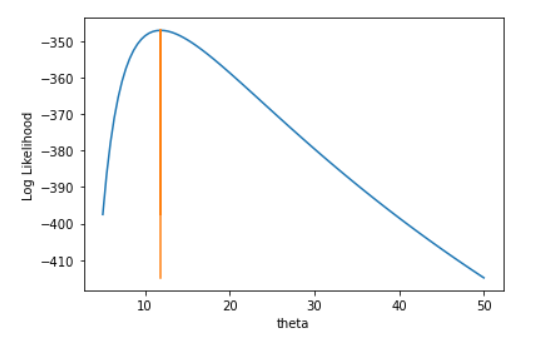
\includegraphics[width=10cm]{fig1.png}
    \caption{Theta vs Log Likelihood}
\end{figure}

The above graph is log likelihood function plotted for various theta. The following variables are chosen - n=100, m=45, t=15.

The graph has global maximum at theta calculated by equation(8)  

\end{document}
